\subsection{Planning with RRT}
\label{sec:planner}

To make use of this information cost function to guide exploration, we consider a sampling-based planning approach that can evaluate the predicted information gain throughout the environment. In addition, we wish to use the occupancy grid that is being updated online (as described in Sect.~\ref{section:occupancy_grid_mapping}) to guide the vehicle around obstacles in the environment. The rapidly-exploring random tree (RRT) algorithm is well suited to planning paths through these types of large environments, and works as follows.
The planner starts from the vehicle's current state and samples a point $x$ in the environment. Using the occupancy grid, we can reject samples that lie in cells with a sufficiently high probability of being occupied. If the sample is valid, we find the closest node in the tree of paths (initially just the vehicle state), where closeness is measured in terms of Euclidean distance, and add a new edge to the tree connecting the sample point to the nearest node.
Then a new sample is drawn and the process repeats to grow a tree of path segments through the environment. This tree-growing process terminates after a specified time, and the minimum cost path is returned.

Figure~\ref{fig:rrt_on_slam_map} shows snapshots of our current implementation of RRT planning over the occupancy grid. As seen in the figure, the edges in the tree are currently direct connections between nodes, but there also exist variants of the algorithm that forward simulate the vehicle dynamics as part of the exploration process~\cite{Kuwata09_TCST}. This approach is traditionally used to ensure dynamic feasibility and dense collision checking. However, this also provides a means for evaluating the information gain along each candidate trajectory. As a result, we can augment the cost of each branch with a metric based on the information cost function from Sect.~\ref{section:explorative_information_cost_function}. This will enable the planner to select the path in the tree that maximizes the predicted information gain.

\begin{figure}[t]
\centering
\begin{subfigure}[b]{0.49\linewidth}
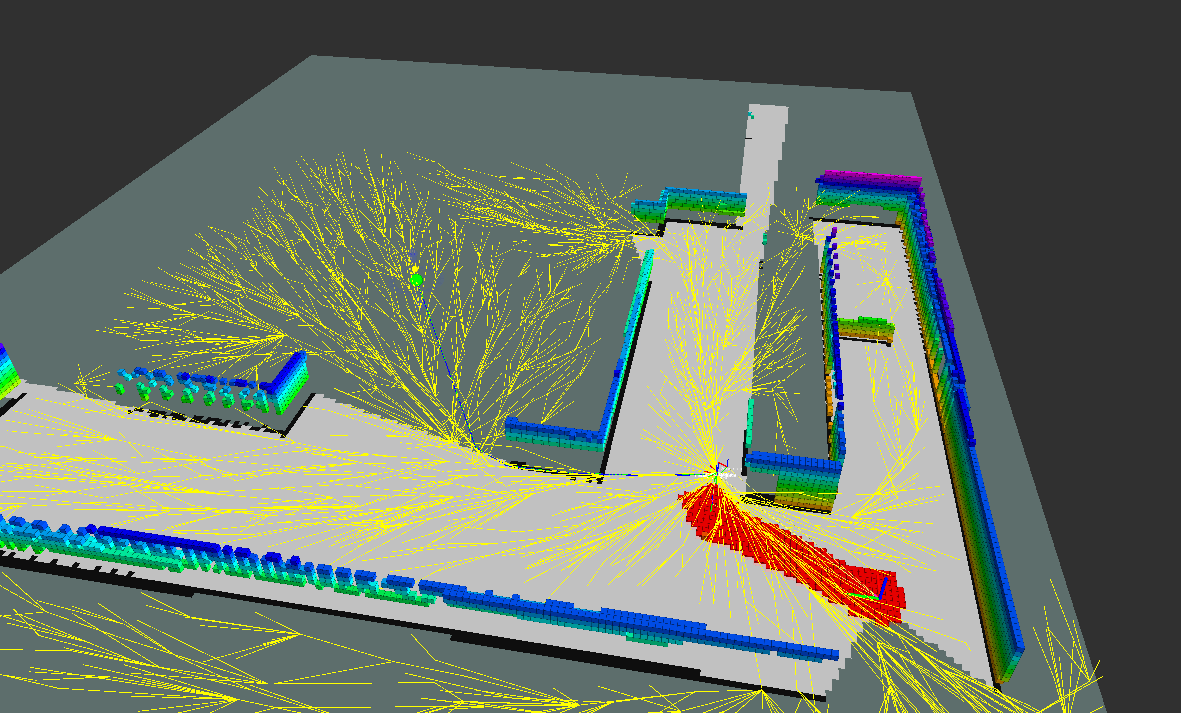
\includegraphics[width=\linewidth]{rrt_on_map}
\label{fig:rrt_on_map}
\end{subfigure}
\begin{subfigure}[b]{0.49\linewidth}
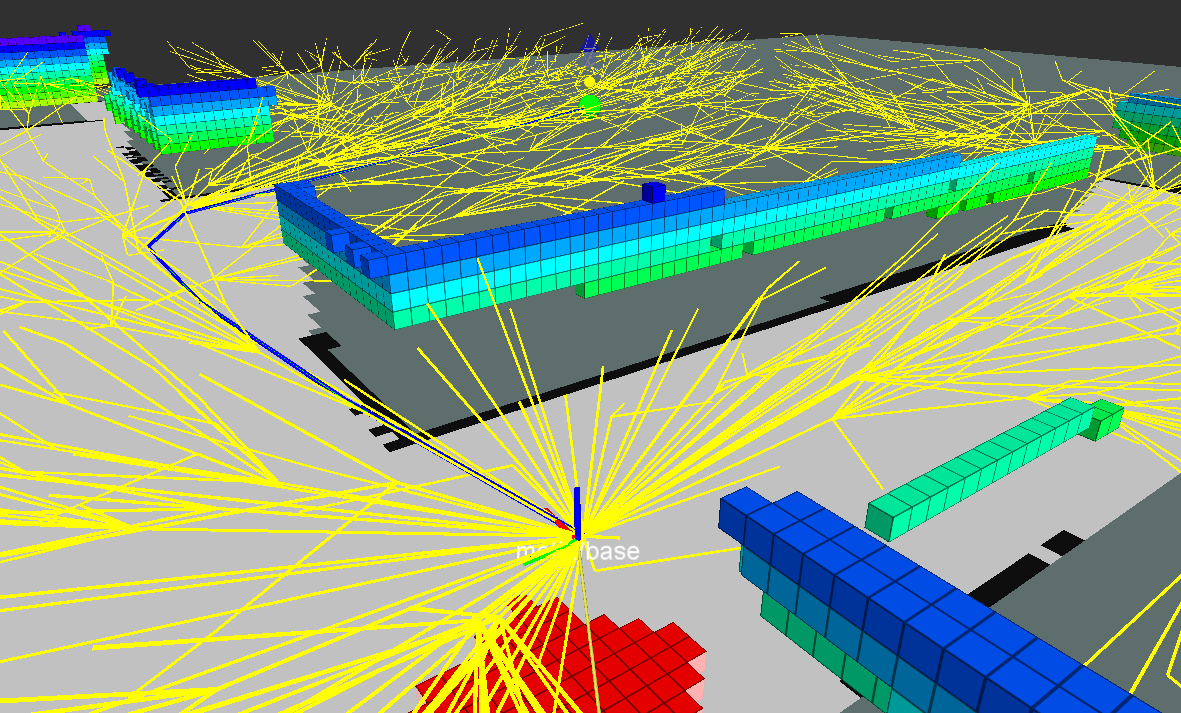
\includegraphics[width=\linewidth]{rrt_on_map_zoom}
\label{fig:rrt_on_map_zoom}
\end{subfigure}
\caption{Snapshots of an RRT exploring the environment defined by the occupancy grid. \label{fig:rrt_on_slam_map}}
\end{figure}
